\documentclass[a4paper,14pt,oneside,openany]{memoir}
\usepackage[left=30mm, right=15mm, top=20mm, bottom=20mm]{geometry}
\usepackage{setspace}
\usepackage{indentfirst}
\usepackage{graphicx}
\usepackage{caption}
\usepackage{hyperref}

% Языковые настройки
\usepackage{polyglossia}
\setdefaultlanguage[indentfirst=true]{russian}
\setotherlanguage{english}

% Шрифты с автоматическим выбором
\usepackage{fontspec}
\defaultfontfeatures{Ligatures=TeX}

\IfFontExistsTF{Times New Roman}
{\setmainfont{Times New Roman}[Script=Cyrillic]}
{\setmainfont{FreeSerif}[Script=Cyrillic]}

\IfFontExistsTF{Arial}
{\setsansfont{Arial}[Script=Cyrillic]}
{\setsansfont{FreeSans}[Script=Cyrillic]}

\IfFontExistsTF{Courier New}
{\setmonofont{Courier New}[Script=Cyrillic]}
{\setmonofont{FreeMono}[Script=Cyrillic]}

% Настройки заголовков
\setsecnumdepth{subsection}
\renewcommand*{\chapterheadstart}{}
\renewcommand*{\printchaptername}{}
\renewcommand*{\chapnumfont}{\normalfont\bfseries}
\renewcommand*{\afterchapternum}{\hspace{1em}}
\renewcommand*{\printchaptertitle}{\normalfont\bfseries\centering\MakeUppercase}
\setbeforesecskip{20pt}
\setaftersecskip{20pt}
\setsecheadstyle{\raggedright\normalfont\bfseries}
\setbeforesubsecskip{20pt}
\setaftersubsecskip{20pt}
\setsubsecheadstyle{\raggedright\normalfont\bfseries}

% Настройки подписей к рисункам
\captionsetup[figure]{
    font=small,
    width=\textwidth,
    name=Рисунок,
    justification=centering,
    aboveskip=10pt,
    belowskip=5pt
}
\captiondelim{ --- }

% Путь к изображениям
\graphicspath{{images/}}

% Параметры отступов и переносов
\parindent=1.25cm
\pagestyle{plain}
\tolerance 1414
\clubpenalty=10000
\widowpenalty=10000

% Гиперссылки
\hypersetup{
    colorlinks=true,
    linktoc=all,
    linktocpage=true,
    linkcolor=blue,
    citecolor=blue
}

\begin{document}

% ========== ТИТУЛЬНЫЙ ЛИСТ ==========
\thispagestyle{empty}
\begin{center}
    МИНИСТЕРСТВО ЦИФРОВОГО РАЗВИТИЯ, СВЯЗИ И МАССОВЫХ КОММУНИКАЦИЙ \\
    РОССИЙСКОЙ ФЕДЕРАЦИИ \vspace{20pt} \\
    Федеральное государственное бюджетное образовательное учреждение \\
    высшего образования \\
    «Сибирский государственный университет телекоммуникаций и информатики» \vspace{20pt} \\
    Кафедра телекоммуникационных систем и вычислительных средств \\
    (ТС и ВС)
\end{center}
\vfill
\begin{center}
    {\normalfont ОТЧЁТ ПО РАСЧЕТНО-ГРАФИЧЕСКОЙ ЗАДАНИЮ} \vspace{10pt} \\
    по дисциплине \\
    {\itshape «Web-Технологии»} \vspace{20pt} \\
    {\normalfont\uppercase{"Создание тестовой видеоплатформы с использованием технологий Python для бэкенда, React JS для фронтенда и Figma для дизайна"}}
\end{center}
\vfill
\noindent Выполнил: \\ {\itshape Студент группы ИКС-531 \hfill В.А. Кириченко} \vspace{10pt} \\
\noindent Проверил: \\ {\itshape Преподаватель кафедры ТС и ВС \hfill А.В. Андреев}
\vfill
\begin{center} Новосибирск, 2026 г. \end{center}

\newpage
\OnehalfSpacing*
\tableofcontents
\newpage
\setcounter{page}{3}

% ========== ОСНОВНОЕ СОДЕРЖАНИЕ ==========
\chapter*{ВВЕДЕНИЕ}
\addcontentsline{toc}{section}{ВВЕДЕНИЕ}
Цель: создать функциональную веб-платформу для потокового видео, где пользователи могут просматривать, загружать и управлять видеоконтентом. Проект должен продемонстрировать ваши навыки в разработке веб-приложений с использованием современного стека технологий и соблюдением принципов \texttt{UI/UX}-дизайна.
    Задачи: 
    \begin{itemize}
        \item Разработать \texttt{API}, использующее \texttt{Django} или \texttt{Flask} для обработки запросов от фронтенда.
        \item Реализовать функционал регистрации и авторизации пользователей с использованием \texttt{JWT}-токенов.
        \item Разработать возможности для загрузки и потокового воспроизведения видео.
        \item Создать базу данных для хранения информации о пользователях, видео и метаданных (используя \texttt{Postgres} или \texttt{MySQL}).
        \item Интеграция с бэкендом для регистрации, входа и воспроизведения видео.
        \item Разработать компоненты для добавления, просмотра и управления видеоконтентом.
        \item Реализовать маршрутизацию (\texttt{React Router}) для навигации между различными страницами приложения.
        \item Проанализировать и понять основные элементы дизайна, включая цветовую палитру, типографику и расположение элементов на странице.
    \end{itemize}

\chapter{FRONTEND}
Фронтенд реализован при помощи фреймворка \texttt{React.js}. 
Каждая из страниц сайта задана собственным файлом \texttt{.jsx}. Т.е папка \texttt{frontend/src/pages} задана 5 файлами:
\begin{enumerate}
    \item \texttt{HomePage.jsx}
    \item \texttt{LoginPage.jsx}
    \item \texttt{RegisterPage.jsx}
    \item \texttt{UploadPage.jsx}
    \item \texttt{VideoPlayerPage.jsx}
\end{enumerate}
Заголовок обозначен в \texttt{src/components/Header.jsx}.
Также имеется файл \texttt{api.js}, регулирующий взаимодействие с бэкендом, в \texttt{App.css}, \texttt{App.jsx}, \texttt{index.css} задаются общие стили и веб-приложение, а \texttt{main.jsx} запускает фронтенд.

\chapter{BACKEND}
Бэкенд работает на \texttt{Django}, в папке \texttt{backend} регулируется хранение данных и взаимодействие с БД PostgreSQL, в папке \texttt{api} задается, как передать данные для фронтенда.
Структура в \texttt{backend}:
\begin{itemize}
    \item \texttt{\_\_init\_\_.py}
    \item \texttt{asgi.py}
    \item \texttt{settings.py}
    \item \texttt{urls.py}
    \item \texttt{wsgi.py}
    \item Директория \texttt{\_\_pycache\_\_}
\end{itemize}
Структура в \texttt{api}:
\begin{itemize}
    \item \texttt{\_\_init\_\_.py}
    \item \texttt{admin.py}
    \item \texttt{apps.py}
    \item \texttt{models.py}
    \item \texttt{serializers.py} 
    \item \texttt{tests.py}
    \item \texttt{urls.py}
    \item \texttt{views.py}
    \item Директория \texttt{\_\_pycache\_\_}
    \item Директория \texttt{migrations}
\end{itemize}

\chapter{ПРИМЕРЫ}
\section{Ссылки}
Ссылка на GitHub:
\href{https://github.com/Eto010/webRGR}{Eto010/webRGR}
Сайт реализован на ВМ.
\section{Изображения}
\begin{figure}[htbp]
    \centering
    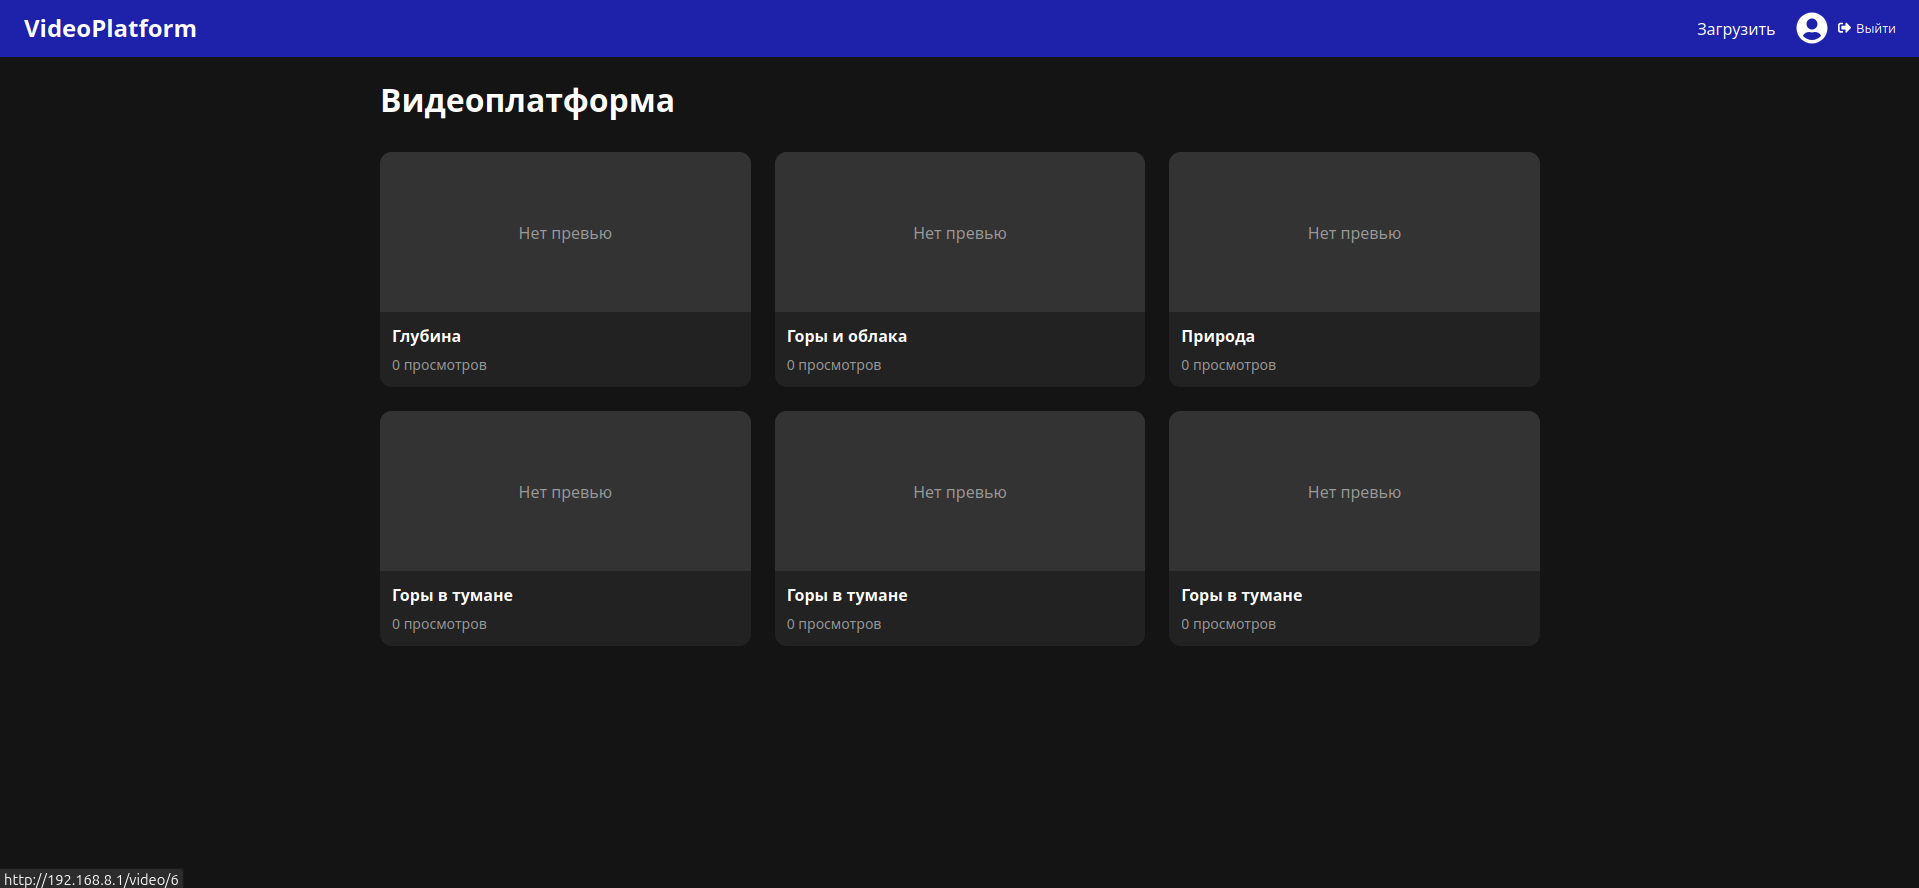
\includegraphics[width=0.85\textwidth, keepaspectratio]{mp.png}
    \caption{Главная страница}
    \label{fig:home}
\end{figure}
\begin{figure}[htbp]
    \centering
    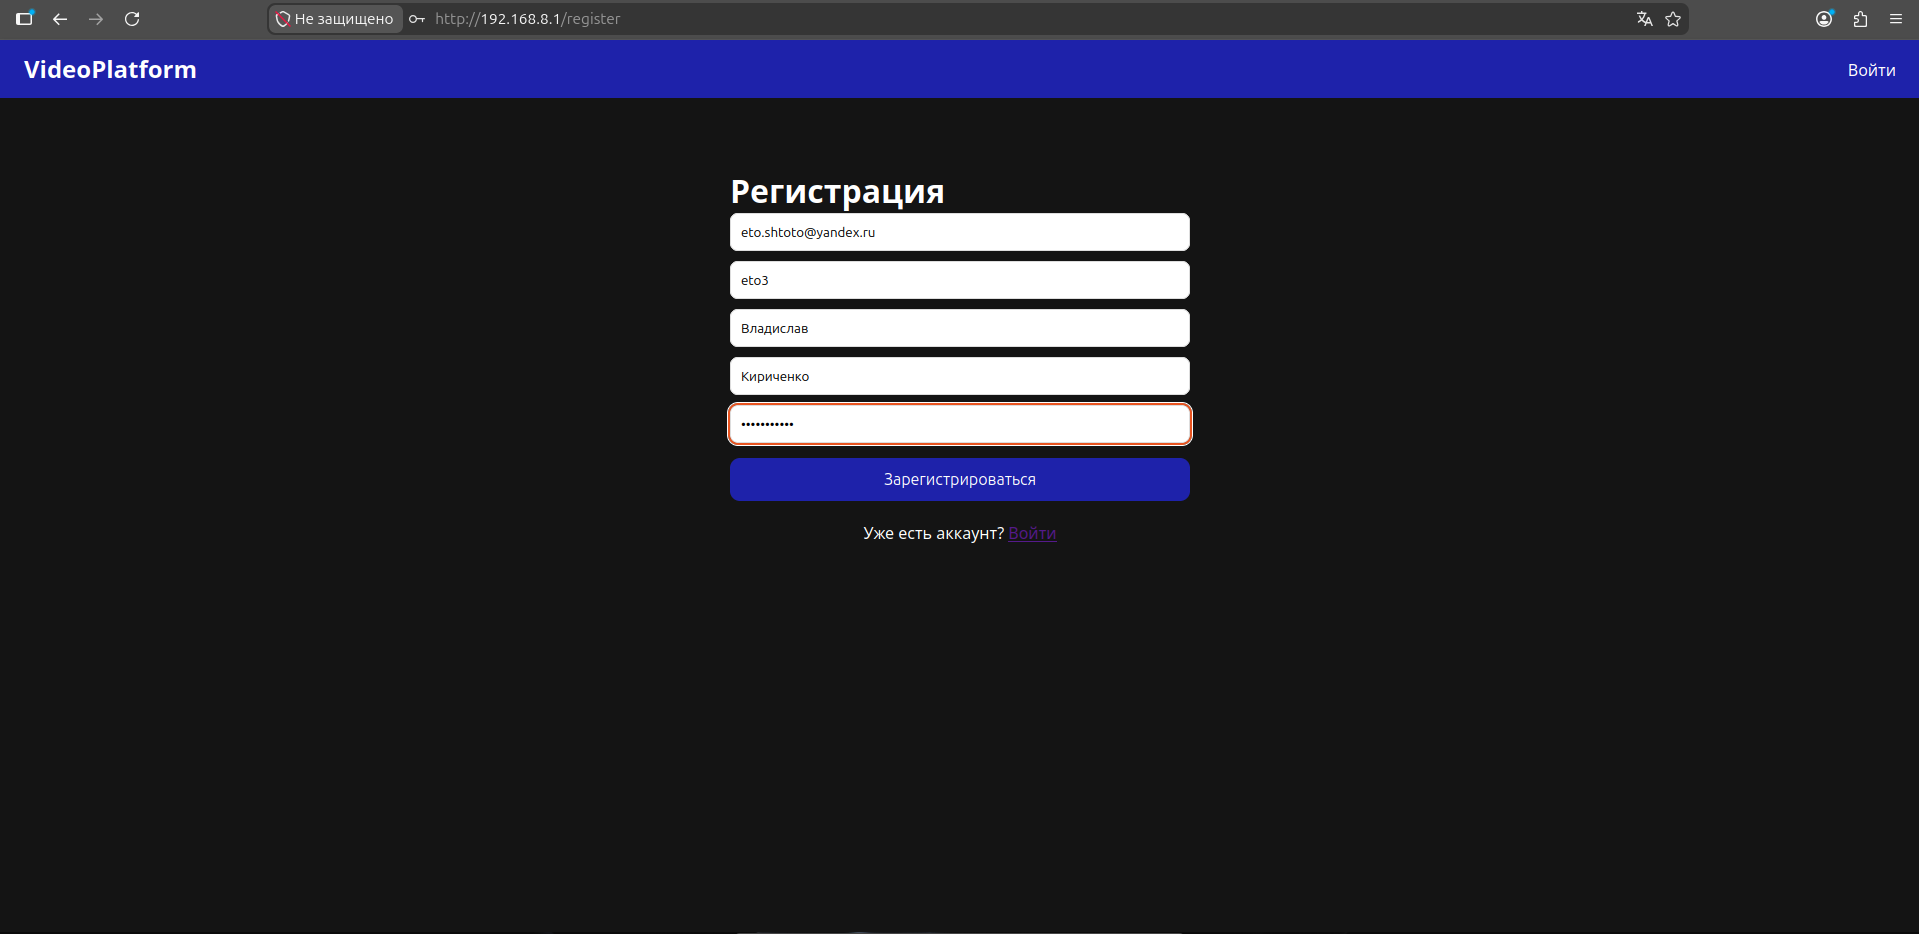
\includegraphics[width=0.85\textwidth, keepaspectratio]{rp.png}
    \caption{Страница регистрации}
    \label{fig:register}
\end{figure}
\begin{figure}[htbp]
    \centering
    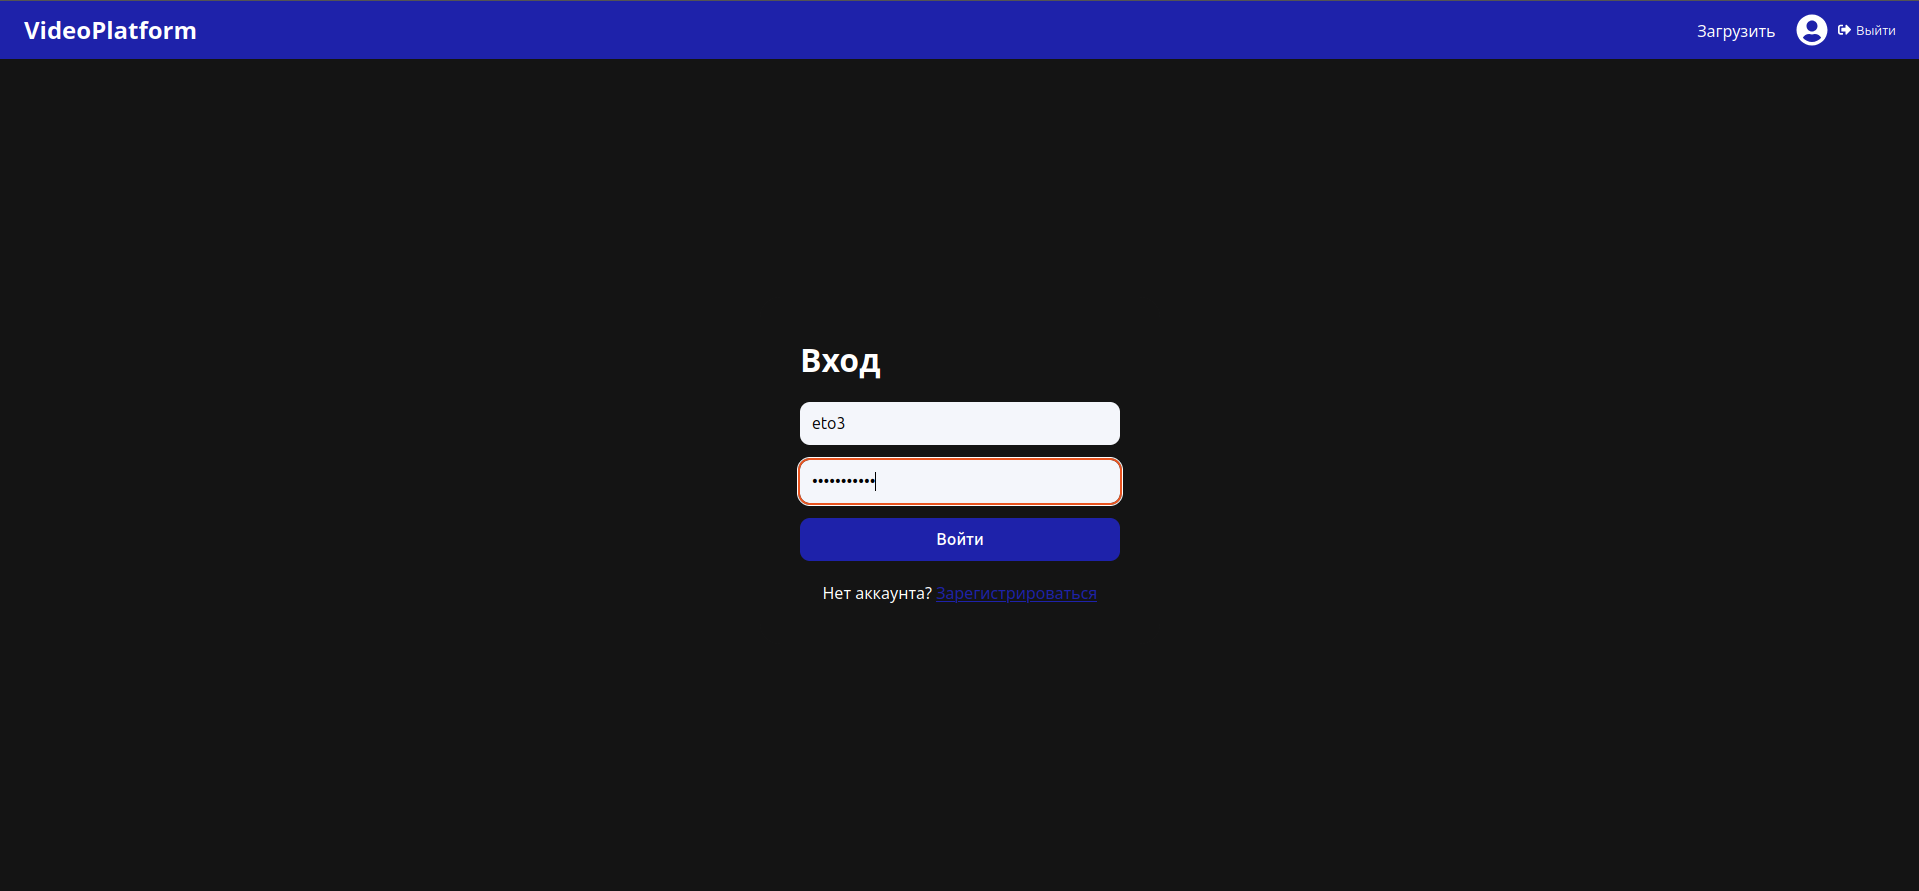
\includegraphics[width=0.85\textwidth, keepaspectratio]{lp.png}
    \caption{Страница входа}
    \label{fig:login}
\end{figure}
\begin{figure}[htbp]
    \centering
    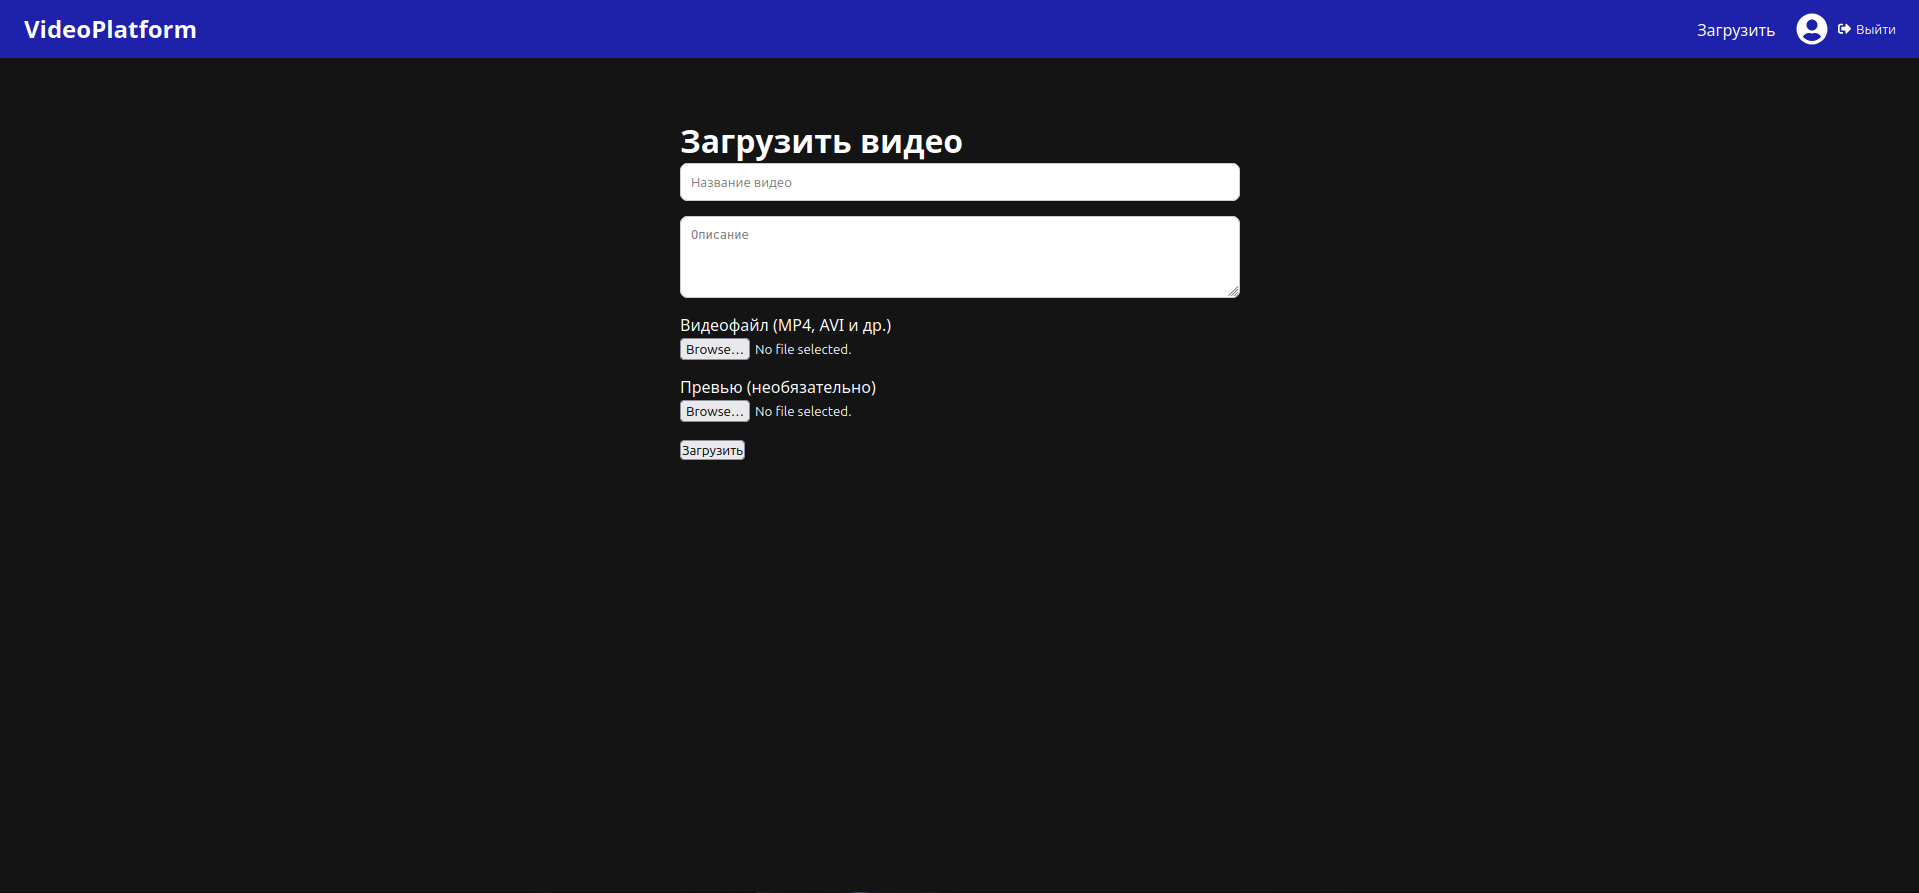
\includegraphics[width=0.85\textwidth, keepaspectratio]{up.png}
    \caption{Страница загрузки}
    \label{fig:upload}
\end{figure}
\begin{figure}[htbp]
    \centering
    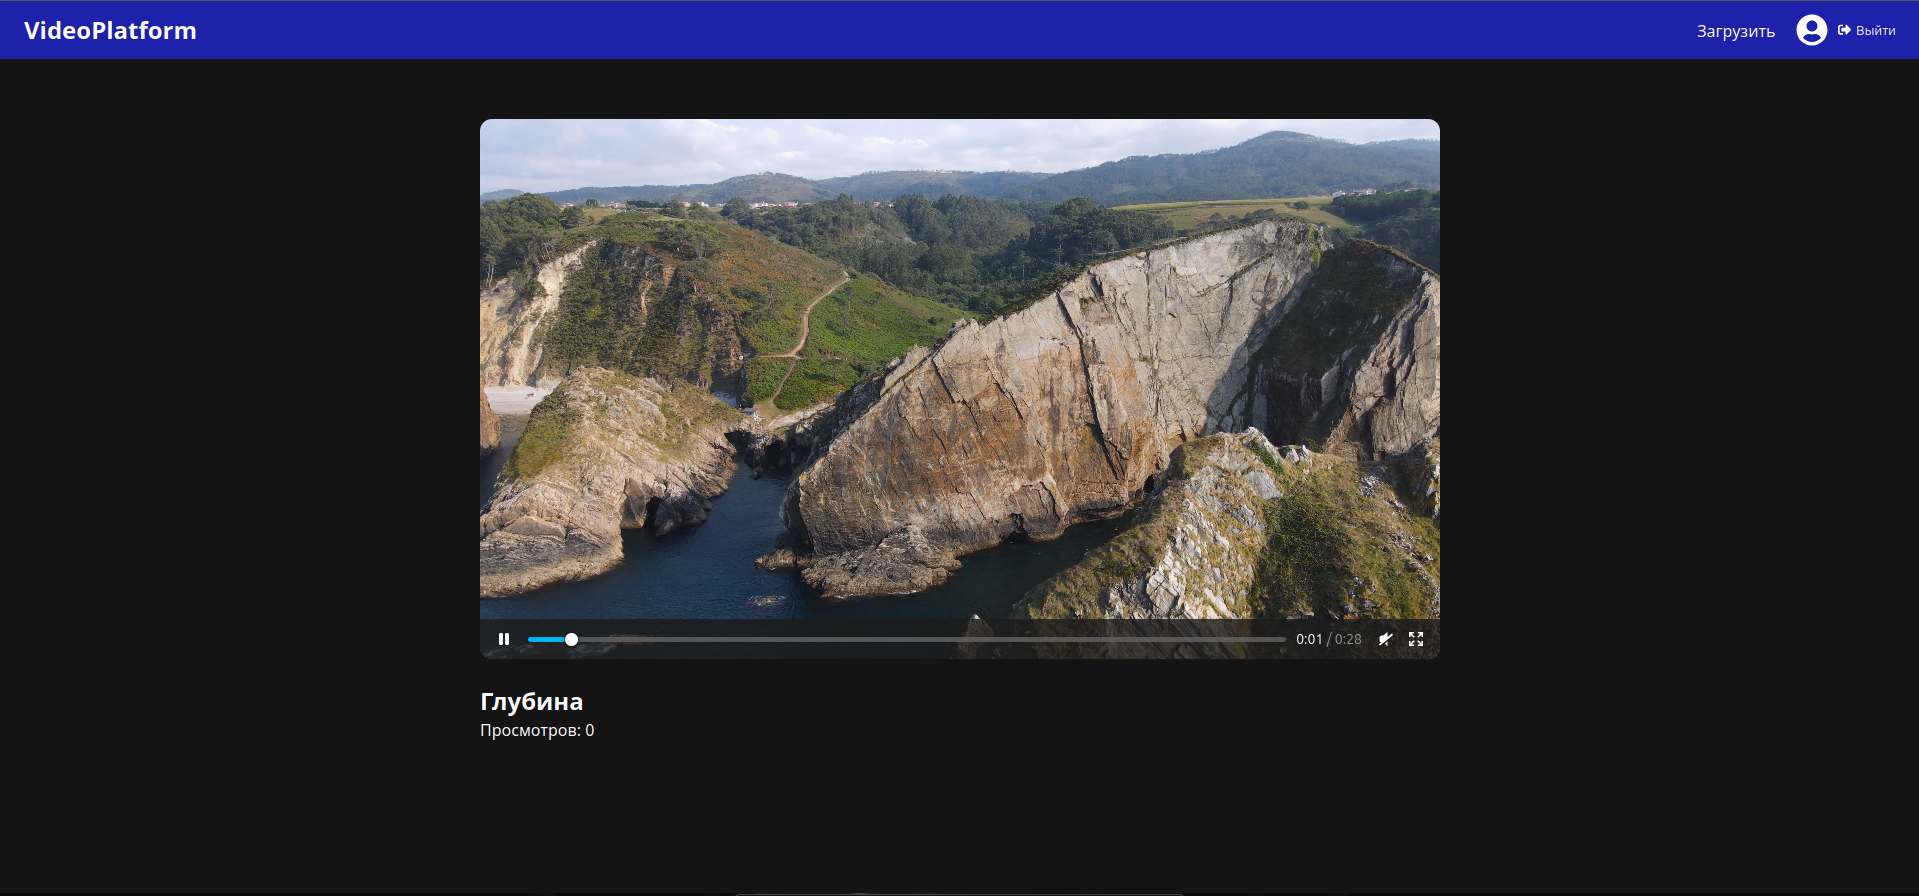
\includegraphics[width=0.85\textwidth, keepaspectratio]{vp.png}
    \caption{Страница воспроизведения видео}
    \label{fig:player}
\end{figure}
\end{document}